\documentclass[conference]{IEEEtran}
\IEEEoverridecommandlockouts

\usepackage{cite}
\usepackage{amsmath,amssymb}
\usepackage{graphicx}
\usepackage{booktabs}
\usepackage{xcolor}
\usepackage{tikz}
\usetikzlibrary{arrows.meta,positioning,calc,decorations.pathreplacing}
\usepackage{pgfplots}
\pgfplotsset{compat=1.17}
\usepackage[hidelinks]{hyperref}
\usepackage{url}

\definecolor{sbblue}{RGB}{31,94,160}
\definecolor{sbred}{RGB}{190,58,48}

\newcommand{\hint}{\texttt{c.li x0,\,$N$}}

\begin{document}

\title{Compiling C for a Hint-Based VLIW: An LLVM Back End for STARBUG on RISC-V Wally\\
{\large Midterm Report}}

\author{
\IEEEauthorblockN{Leo Marek, Gregory Chekler\IEEEauthorrefmark{1}, Jing Jing Chen\IEEEauthorrefmark{1}, Elliot Chae\IEEEauthorrefmark{1}, Ethan Carr\IEEEauthorrefmark{1}, and Ray Simar}
\IEEEauthorblockA{Department of Electrical and Computer Engineering, Rice University, Houston, TX, USA\\
\{lnm7, gsc8, jc165, ejc12, ehc6, ray.simar\}@rice.edu\qquad \IEEEauthorrefmark{1}Equal contribution}
}

\maketitle

\begin{abstract}
STARBUG is a four-lane VLIW extension to the CORE-V Wally RISC-V core in which each bundle is announced by the compressed instruction \hint, an architectural no-op. The same binary therefore runs unmodified on a stock RV32C core and in parallel on STARBUG. Our earlier evaluation relied on hand-scheduled assembly, which left open whether a compiler can target the design at all. This report describes midterm progress on an LLVM back end that forms bundles automatically from ordinary C. It combines a post-register-allocation packetizer that keeps every bundle correct under both parallel and sequential execution, an I-cache-line-aware layout pass, and a static bundle verifier. In RTL simulation of five CMSIS-DSP kernels, compiled code reaches a 1.40$\times$ geometric-mean speedup over scalar code versus 1.47$\times$ for hand scheduling, recovering 95.6\% of the hand-scheduled gain. No compiled binary contains an illegal bundle, whereas four of ten hand-scheduled binaries do.
\end{abstract}

\begin{IEEEkeywords}
RISC-V, VLIW, LLVM, instruction scheduling, DSP, CORE-V Wally
\end{IEEEkeywords}

\section{Introduction}
Embedded DSP workloads need high instruction throughput under tight power and area budgets. Superscalar and out-of-order cores find instruction-level parallelism (ILP) dynamically, but at a hardware cost that is hard to justify in a small core. VLIW machines move scheduling to the compiler~\cite{fisher-vliw-1983}, but traditional VLIW encodings break binary compatibility, which has limited their adoption in the RISC-V ecosystem.

STARBUG takes a hybrid approach. A RISC-V HINT, the 16-bit \hint{} with $1\le N\le 4$~\cite{riscv-unpriv}, tells a modified CORE-V Wally core~\cite{corev-wally,harris-socdesign-2025} that the next $N$ instructions are independent and may issue together. A standard core sees a write to \texttt{x0} and treats it as a no-op. Last semester we modeled the bundle semantics in Google's MPACT simulator, implemented four-lane issue in Wally RTL, extended the floating-point (FP) datapath to all lanes, and synthesized the design for a Xilinx VCU108 FPGA. Hand-scheduled integer kernels ran 1.24--1.51$\times$ faster than scalar code.

Reviewers of that work raised one main objection: for an ISA extension whose selling point is that existing toolchains keep working, hand-scheduled kernels show the hardware's upper bound but say nothing about whether a compiler can produce valid bundles. This semester's objective is to answer that question. Our goals are to (i)~build an LLVM~\cite{lattner-llvm-2004} back end that emits STARBUG bundles from unmodified C, (ii)~measure it against hand scheduling on the same RTL, and (iii)~make bundle legality checkable, since the hardware does not check it. This report covers the architecture briefly and focuses on the compiler.

\section{Methods}

\subsection{STARBUG Architecture Overview}
Fig.~\ref{fig:arch} summarizes the design. The instruction fetch unit (IFU) recognizes the hint before decompression, extracts up to four 16- or 32-bit payload instructions from the current I-cache line, and dispatches them to four lanes that share a widened integer register file (8 read / 4 write ports) and a widened FP register file. Lane~0 is a full Wally execution unit. Worker lanes~1--3 handle integer, multiply, and FP arithmetic, but their branch-redirect and load/store paths are disconnected. The single load/store unit (LSU) therefore limits each bundle to one memory operation, which must be in lane~0. The fetch unit may also \emph{decline} a bundle: if $N>4$, if the bundle crosses a 64-byte I-cache line, or if a branch lands inside it. In that case the hint retires as a no-op and the payload runs sequentially. To save area there is no interlock: an intra-bundle dependence or a worker-lane memory operation silently produces a wrong result, not a fault.

\begin{figure}[t]
\centering
% Fig. 1 -- STARBUG bundle encoding and lane structure (drawn to fit one IEEE column, 88 mm).
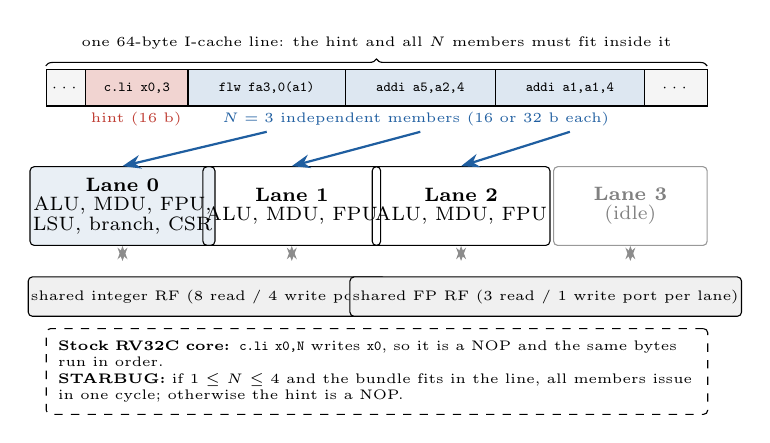
\begin{tikzpicture}[
  x=1mm, y=1mm,
  font=\scriptsize,
  >=Stealth,
  word/.style={draw, minimum height=4.6mm, inner sep=0pt, font=\ttfamily\tiny, anchor=west},
  lane/.style={draw, rounded corners=1.5pt, minimum height=10mm, minimum width=19.5mm, align=center, inner sep=1pt},
  rf/.style={draw, rounded corners=1.5pt, fill=black!6, minimum height=5mm, minimum width=41mm, align=center, inner sep=1pt, font=\tiny},
]
% ---- fetch line (x = 0..84) -------------------------------------------
\node[word, fill=black!4,  minimum width=5mm]  (pre)  at (0,0)  {$\cdots$};
\node[word, fill=sbred!22, minimum width=13mm] (h)    at (5,0)  {c.li x0,3};
\node[word, fill=sbblue!15,minimum width=20mm] (p0)   at (18,0) {flw fa3,0(a1)};
\node[word, fill=sbblue!15,minimum width=19mm] (p1)   at (38,0) {addi a5,a2,4};
\node[word, fill=sbblue!15,minimum width=19mm] (p2)   at (57,0) {addi a1,a1,4};
\node[word, fill=black!4,  minimum width=8mm]  (rest) at (76,0) {$\cdots$};
\draw[decorate, decoration={brace, amplitude=2.5pt}] (0,2.8) -- (84,2.8)
  node[midway, above=2.5pt, font=\tiny] {one 64-byte I-cache line: the hint and all $N$ members must fit inside it};
\node[font=\tiny, text=sbred]  at (11.5,-3.9) {hint (16 b)};
\node[font=\tiny, text=sbblue] at (47,-3.9) {$N=3$ independent members (16 or 32 b each)};

% ---- lanes ------------------------------------------------------------
\node[lane, fill=sbblue!10] (l0) at (9.75,-15)  {\textbf{Lane 0}\\[-1pt]ALU, MDU, FPU,\\[-1pt]LSU, branch, CSR};
\node[lane]                 (l1) at (31.25,-15) {\textbf{Lane 1}\\[-1pt]ALU, MDU, FPU};
\node[lane]                 (l2) at (52.75,-15) {\textbf{Lane 2}\\[-1pt]ALU, MDU, FPU};
\node[lane, draw=black!40, text=black!50] (l3) at (74.25,-15) {\textbf{Lane 3}\\[-1pt](idle)};
\draw[->, sbblue, thick] (p0.south) ++(0,-3.2) -- (l0.north);
\draw[->, sbblue, thick] (p1.south) ++(0,-3.2) -- (l1.north);
\draw[->, sbblue, thick] (p2.south) ++(0,-3.2) -- (l2.north);

% ---- register files ---------------------------------------------------
\node[rf] (irf) at (20.5,-26.5) {shared integer RF (8 read / 4 write ports)};
\node[rf] (frf) at (63.5,-26.5) {shared FP RF (3 read / 1 write port per lane)};
\foreach \l in {l0,l1,l2,l3} { \draw[<->, black!45] (\l.south) -- ++(0,-1.9); }

% ---- behaviour note ---------------------------------------------------
\node[draw, dashed, rounded corners=1.5pt, align=left, text width=81mm, inner sep=1.5mm,
      anchor=north west, font=\tiny] at (0,-30.5)
  {\textbf{Stock RV32C core:} \texttt{c.li x0,N} writes \texttt{x0}, so it is a NOP and the same bytes run in order.\\
   \textbf{STARBUG:} if $1\le N\le 4$ and the bundle fits in the line, all members issue in one cycle; otherwise the hint is a NOP.};
\end{tikzpicture}

\caption{STARBUG bundle encoding and lane structure. The three-instruction bundle is taken from the hand-scheduled biquad kernel; its single memory operation is placed in lane~0.}
\label{fig:arch}
\end{figure}

\subsection{Compiler Obligations}
Because a bundle is a request that the hardware may refuse, the compiler must satisfy three obligations that a conventional VLIW compiler does not face:
\begin{enumerate}
\item \emph{Dual correctness.} Every bundle must be correct both as a parallel issue group and as a sequential instruction stream, since declined bundles and stock cores execute the bytes in order (Table~\ref{tab:hazards}).
\item \emph{Lane legality without a safety net.} Memory, control-flow, CSR, and PC-relative instructions must be in lane~0, with at most one memory operation per bundle.
\item \emph{Placement.} A bundle exists only if it fits within one I-cache line, so whether it is used depends on where the instructions end up in the final binary. Placement constraints of this kind are otherwise found only in explicitly parallel encodings such as IA-64~\cite{schlansker-epic-2000} and the TI C6x~\cite{ti-c6000}.
\end{enumerate}

\begin{table}[t]
\centering
\caption{Register hazards between members of one bundle}
\label{tab:hazards}
\footnotesize\setlength{\tabcolsep}{4pt}
\begin{tabular}{@{}lll@{}}
\toprule
Hazard & Parallel issue & Sequential fallback (if reordered)\\
\midrule
RAW & unsafe (no same-cycle bypass) & unsafe\\
WAW & unsafe (no defined winner) & unsafe\\
WAR & safe (all lanes read first) & unsafe once order changes\\
\bottomrule
\end{tabular}
\end{table}

\subsection{LLVM Back End}
The back end is a fork of LLVM targeting \texttt{riscv32} with \texttt{-mcpu=starbug-vliw}. Fig.~\ref{fig:compiler}(a) shows where its passes run in the code generator.

\emph{Packetizer.} Bundles are formed after register allocation, because legality depends on physical registers. RAW and WAW conflicts always end a packet. WAR is the subtle case: it is harmless in parallel, but becomes illegal if the packetizer reorders instructions. We therefore accept WAR pairs only while the packet still follows the original program order. Instructions are classified by opcode and by \texttt{mayLoad}/\texttt{mayStore} flags rather than by mnemonic, and FP operations may use any lane, matching the RTL. An unrecognized instruction defaults to lane~0, which is always safe.

\emph{Bundle layout pass.} This pass runs last, after compression, branch relaxation, and pseudo-instruction expansion, because byte offsets are not final until then. It tracks the emitted size of every instruction, including branches that the assembler will compress, and splits any bundle that would cross a 64-byte line into two bundles at the boundary (Fig.~\ref{fig:compiler}(b)). Splitting never moves an instruction, adds no padding, and preserves program order. Any subset of an independent set is still independent, so both halves remain legal.

\emph{Unroll policy.} Spills are memory operations that compete for the single lane-0 LSU, so we cap unrolling at a factor of 8 (maximum 16), the best point in our sweep.

\begin{figure}[t]
\centering
\resizebox{\columnwidth}{!}{% Fig. 2 -- (a) STARBUG passes in the LLVM RISC-V code generator,
%          (b) the I-cache-line layout pass splitting a straddling bundle.
% Drawn to fit one IEEE column (88 mm).
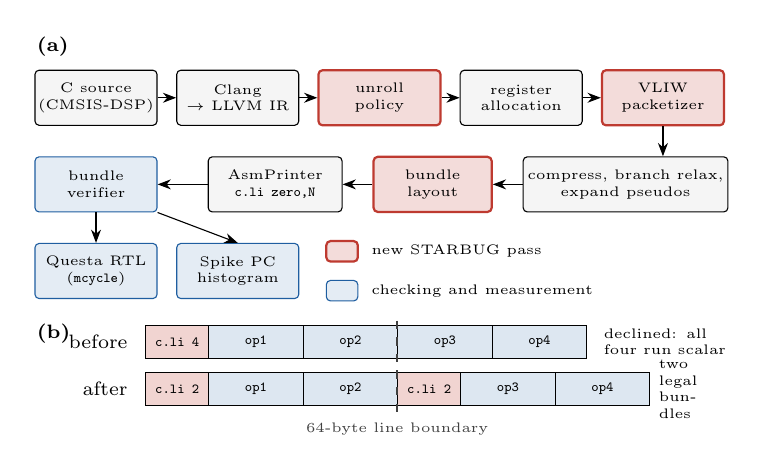
\begin{tikzpicture}[
  x=1mm, y=1mm,
  font=\tiny,
  >=Stealth,
  stage/.style={draw, rounded corners=1.5pt, minimum height=7mm, align=center, inner sep=1pt, fill=black!4},
  new/.style={stage, fill=sbred!18, draw=sbred, thick},
  tool/.style={stage, fill=sbblue!12, draw=sbblue},
  word/.style={draw, minimum height=4.2mm, inner sep=0pt, font=\ttfamily\tiny, anchor=west},
]
% ---- (a) row 1 ---------------------------------------------------------
\node[font=\bfseries\scriptsize, anchor=west] at (-1,6.5) {(a)};
\node[stage, minimum width=15.5mm] (c)  at (7.75,0)  {C source\\(CMSIS-DSP)};
\node[stage, minimum width=15.5mm] (ir) at (25.75,0) {Clang\\$\to$ LLVM IR};
\node[new,   minimum width=15.5mm] (un) at (43.75,0) {unroll\\policy};
\node[stage, minimum width=15.5mm] (ra) at (61.75,0) {register\\allocation};
\node[new,   minimum width=15.5mm] (pk) at (79.75,0) {VLIW\\packetizer};
\draw[->] (c) -- (ir); \draw[->] (ir) -- (un); \draw[->] (un) -- (ra); \draw[->] (ra) -- (pk);
% ---- (a) row 2 (right to left) ---------------------------------------
\node[stage, minimum width=26mm] (late) at (75,-11)  {compress, branch relax,\\expand pseudos};
\node[new,   minimum width=15mm] (lay)  at (50.5,-11) {bundle\\layout};
\node[stage, minimum width=17mm] (asm)  at (30.5,-11) {AsmPrinter\\\texttt{c.li zero,N}};
\node[tool,  minimum width=15.5mm] (ver) at (7.75,-11) {bundle\\verifier};
\draw[->] (pk.south) -- (pk.south |- late.north);
\draw[->] (late) -- (lay); \draw[->] (lay) -- (asm); \draw[->] (asm) -- (ver);
% ---- (a) row 3 ---------------------------------------------------------
\node[tool, minimum width=15.5mm] (sim) at (7.75,-22)  {Questa RTL\\(\texttt{mcycle})};
\node[tool, minimum width=15.5mm] (spk) at (25.75,-22) {Spike PC\\histogram};
\draw[->] (ver) -- (sim); \draw[->] (ver.south east) -- (spk.north);
\node[new,  minimum width=4mm, minimum height=2.6mm] (k1) at (39,-19.5) {};
\node[anchor=west] at (41.5,-19.5) {new STARBUG pass};
\node[tool, minimum width=4mm, minimum height=2.6mm] (k2) at (39,-24.5) {};
\node[anchor=west] at (41.5,-24.5) {checking and measurement};

% ---- (b) layout split --------------------------------------------------
\node[font=\bfseries\scriptsize, anchor=west] at (-1,-30) {(b)};
\node[anchor=east, font=\scriptsize] at (13,-31) {before};
\node[anchor=west, align=left, text width=17mm] at (71,-31) {declined: all four run scalar};
\node[word, fill=sbred!22,  minimum width=8mm]  at (14,-31) {c.li 4};
\node[word, fill=sbblue!15, minimum width=12mm] at (22,-31) {op1};
\node[word, fill=sbblue!15, minimum width=12mm] at (34,-31) {op2};
\node[word, fill=sbblue!15, minimum width=12mm] at (46,-31) {op3};
\node[word, fill=sbblue!15, minimum width=12mm] at (58,-31) {op4};
\node[anchor=east, font=\scriptsize] at (13,-37) {after};
\node[anchor=west, align=left, text width=8mm, inner sep=0.5pt] at (79,-37) {two legal bundles};
\node[word, fill=sbred!22,  minimum width=8mm]  at (14,-37) {c.li 2};
\node[word, fill=sbblue!15, minimum width=12mm] at (22,-37) {op1};
\node[word, fill=sbblue!15, minimum width=12mm] at (34,-37) {op2};
\node[word, fill=sbred!22,  minimum width=8mm]  at (46,-37) {c.li 2};
\node[word, fill=sbblue!15, minimum width=12mm] at (54,-37) {op3};
\node[word, fill=sbblue!15, minimum width=12mm] at (66,-37) {op4};
\draw[dashed, thick, black!75] (46,-28.3) -- (46,-40) node[below, font=\tiny] {64-byte line boundary};
\end{tikzpicture}
}
\caption{(a) STARBUG passes (red) in the LLVM RISC-V code generator and the checking flow (blue). (b) The layout pass splits a bundle that would cross an I-cache line; no instruction moves and no padding is added.}
\label{fig:compiler}
\end{figure}

\subsection{Verification and Evaluation}
\emph{Bundle verifier.} A standalone checker reconstructs every bundle from the final ELF encodings. It rejects intra-bundle RAW/WAW conflicts, illegal lane assignments, and hints with $N>4$. The checker uses the same hardware contract, read directly from the RTL, as the back end.

\emph{Workloads and measurement.} We use five CMSIS-DSP~\cite{cmsis-dsp} float32 kernels (FIR, biquad, LMS, DCT-IV, real FFT) and build each one three ways: GCC \texttt{-O3} scalar (\texttt{rv32gc}), hand-scheduled assembly, and STARBUG LLVM. We report cycles in the kernel region (\texttt{mcycle}) from full-RTL Questa simulation, including caches and LSU contention. For bundle coverage and ILP, we join Spike~\cite{spike} PC histograms with the static bundle map. This is valid because the hint is a no-op on Spike. Each kernel also checks its output signal-to-noise ratio (SNR) against a golden reference.

\section{Results (Partial)}
\emph{Speedup.} Fig.~\ref{fig:speedup} compares compiled and hand-scheduled code. Compiled code reaches a 1.402$\times$ geometric mean over scalar, versus 1.465$\times$ for hand scheduling, so the compiler recovers 95.6\% of the hand-scheduled speedup with no manual annotation. On \texttt{rfft512} the compiled build is 6.9\% \emph{faster} than the hand-scheduled one. The hand-written hints cover only the code path taken by 2048-point transforms, so at 512 points the hand-scheduled hot function \texttt{arm\_radix8\_butterfly\_f32} runs entirely unbundled (0.0\% coverage, ILP 1.00). The compiler covers both paths (81.4\% coverage, ILP 2.32). The largest gap is \texttt{lms}, where the compiler reaches 85\% of the hand speedup.

\begin{figure}[t]
\centering
% Fig. 3 -- Compiler vs. hand-scheduled speedup over the scalar build.
% Data: llvm_results/paper/02-results.md, Table 1 (V2, layout pass on).
% Cycles are Questa RTL simulation of the kernel region (mcycle).
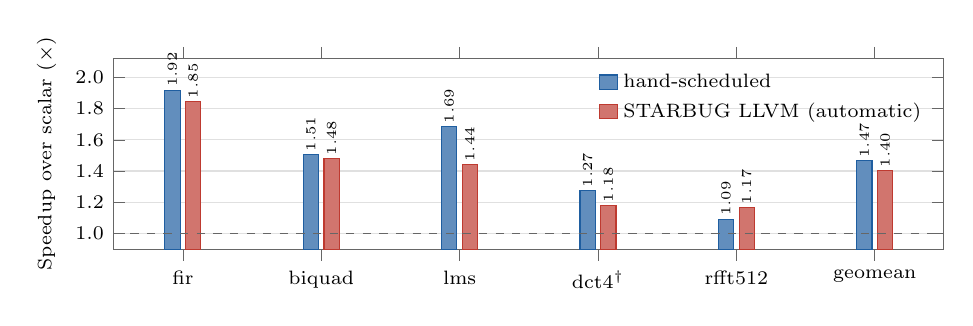
\begin{tikzpicture}
\begin{axis}[
  width=\columnwidth, height=40mm,
  ybar, bar width=5.5pt,
  ylabel={Speedup over scalar ($\times$)},
  ylabel style={font=\scriptsize},
  symbolic x coords={fir,biquad,lms,dct4$^\dagger$,rfft512,geomean},
  xtick=data,
  x tick label style={font=\scriptsize},
  y tick label style={font=\scriptsize},
  ymin=0.9, ymax=2.12,
  ytick={1.0,1.2,1.4,1.6,1.8,2.0},
  ymajorgrids, grid style={black!12},
  enlarge x limits=0.10,
  axis line style={black!60},
  tick style={black!60},
  legend cell align=left,
  yticklabel style={/pgf/number format/.cd, fixed, precision=1, zerofill},
  legend style={font=\scriptsize, draw=none, fill=none, at={(0.99,0.98)}, anchor=north east,
                legend columns=1, /tikz/every even column/.append style={column sep=4pt}},
  legend image code/.code={\draw[#1] (0cm,-0.08cm) rectangle (0.22cm,0.1cm);},
  nodes near coords,
  every node near coord/.append style={font=\tiny, rotate=90, anchor=west, inner sep=1pt,
                                       /pgf/number format/.cd, fixed, precision=2, zerofill},
]
\addplot[draw=sbblue, fill=sbblue!70] coordinates {
  (fir,1.917) (biquad,1.505) (lms,1.685) (dct4$^\dagger$,1.274) (rfft512,1.091) (geomean,1.465)};
\addlegendentry{hand-scheduled}
\addplot[draw=sbred, fill=sbred!70] coordinates {
  (fir,1.846) (biquad,1.479) (lms,1.439) (dct4$^\dagger$,1.180) (rfft512,1.167) (geomean,1.402)};
\addlegendentry{STARBUG LLVM (automatic)}
\draw[black!60, dashed] (rel axis cs:0,0.0820) -- (rel axis cs:1,0.0820);
\end{axis}
\end{tikzpicture}

\caption{Kernel-region speedup over the GCC \texttt{-O3} scalar build (Questa RTL, layout pass enabled). Dashed line: scalar. $^\dagger$\texttt{dct4} misses its SNR threshold in every build, including clang without the packetizer (Sec.~\ref{sec:discussion}).}
\label{fig:speedup}
\end{figure}

\emph{Legality.} Across all twenty binaries, the verifier finds illegal bundles in 4 of 10 hand-scheduled binaries and in none of the 10 compiled ones. The defects include a branch in a worker lane on a live path in \texttt{arm\_dct4\_f32}. Because worker lanes cannot redirect the PC, the branch falls through into an unrolled body and causes a silent out-of-bounds access, which the kernel's output check happens to miss. A second defect is an intra-bundle RAW pair in \texttt{arm\_bitreversal\_16}.

\emph{Effect of individual fixes.} Table~\ref{tab:ablation} isolates the main back-end fixes, measured in statically bundled instructions per kernel. The largest effect came from debug information. Each \texttt{DBG\_VALUE} ended the packet in progress, so building with \texttt{-g} removed about three quarters of all bundling. Hand-written assembly was unaffected, so this defect lowered only the compiler's numbers. The layout pass adds 1.98\% geometric-mean speedup (up to 4.4\% on biquad). Disassembly with hints removed shows that the pass changes only PC-relative immediates.

\begin{table}[t]
\centering
\caption{Statically bundled instructions before and after each back-end fix, and speedup from the layout pass}
\label{tab:ablation}
\footnotesize
\begin{tabular}{@{}llrr@{}}
\toprule
Fix & Kernel & Before & After\\
\midrule
Debug instructions ignored (\texttt{-g}) & biquad & 40 & 144\\
FP allowed in worker lanes & biquad & 69 & 155\\
Intra-bundle WAR accepted & cfft\_radix8 & 195 & 237\\
Line-aware layout (speedup) & 5-kernel geomean & --- & +1.98\%\\
\bottomrule
\end{tabular}
\end{table}

\section{Discussion (Partial)}
\label{sec:discussion}
The midterm results suggest that STARBUG can be targeted by a compiler. Automatic bundling reaches most of the hand-scheduled performance, covers code that hand scheduling missed, and is the only producer in our study whose output passes the legality check. The remaining gap has two known causes. First, bundles cannot span basic blocks. In biquad, the pointer updates that the hand-written code folds into FP bundles sit past a branch in compiled code (ILP 2.14 versus 2.61), which global scheduling~\cite{bernstein-rodeh-1991,hwu-superblock-1993} would address. Second, there is no modulo scheduling~\cite{rau-modulo-1994}. FIR and LMS are limited by the single LSU, so the best schedule pairs each load with the previous tap's multiply-add. That pairing requires software pipelining, and more unrolling does not help.

Two findings concern the toolchain rather than the architecture. Linker relaxation removes bytes after the layout pass has run, which invalidates its offsets. Disabling relaxation makes the pass more effective, but costs FIR about 6\% on its own. Layout-sensitive hints therefore need support across the whole toolchain, including the linker. Also, an estimate that line-crossing bundles cost FIR 20\% of runtime proved wrong: removing most of them gained 0.34\%. Decline rates are not a performance model, so we report RTL cycles.

Several threats to validity remain, and they set our plan for the rest of the semester. Correctness currently rests on per-kernel SNR checks and the static verifier. LMS and rfft pass by only 1\,dB, so we will add lockstep comparison against Spike. The scalar baseline uses GCC rather than clang, so part of the speedup may come from the different compiler; a clang scalar build will isolate the effect of bundling. \texttt{dct4\_512} misses its 118\,dB threshold in every configuration, including clang with no packetizer (110\,dB), because the threshold was calibrated against GCC's floating-point contraction. We will recalibrate it. Our FPGA area figures appear to compare integer-only and FP-enabled STARBUG rather than stock Wally, so we will re-synthesize against an unmodified \texttt{rv32gc} configuration. Finally, the workload set is narrow. We will extend the evaluation to 13 integer and control-heavy kernels and to the five benchmark variants not yet measured with the layout pass, and we will replace the static branch-size guess in the layout pass with an iterative branch-distance model.

\section*{Acknowledgements}
We thank David Harris, James Stine, and the OpenHW Group for the open-source CORE-V Wally core, the developers of Google MPACT and Spike, and Rice University ECE for support. Generative AI tools were used to help write code, debug, and draft and edit this report. The authors reviewed all such content and take full responsibility for it.

\section*{CRediT Author Statement}
Roles follow the CRediT taxonomy~\cite{credit}. \textbf{Leo Marek:} Conceptualization, Methodology, Software (LLVM back end, verifier), Validation, Formal Analysis, Investigation, Visualization, Writing -- Original Draft, Writing -- Review \& Editing. \textbf{Gregory Chekler, Jing Jing Chen, Elliot Chae, Ethan Carr:} Methodology, Validation, Investigation, Writing -- Review \& Editing. \textbf{Ray Simar:} Conceptualization, Supervision, Resources.

\bibliographystyle{IEEEtran}
\bibliography{references}

\end{document}
